\documentclass[12pt]{scrreprt}
\usepackage{graphicx}
\usepackage[font=small,labelfont=bf]{caption} 
\usepackage{titlepic}
\usepackage{wrapfig}

\graphicspath{{./img/}}

% Title Page
\title{Deliverable \#1}
\author{Team D\'evlopp}
\titlepic{
\includegraphics[width=0.6\textwidth]{logo.png}}


\begin{document}
\maketitle
\tableofcontents

\section{The team}
We are team D\'evlopp. Our logo can be seen on the title page.

\subsection{Team photos}
\begin{center}
	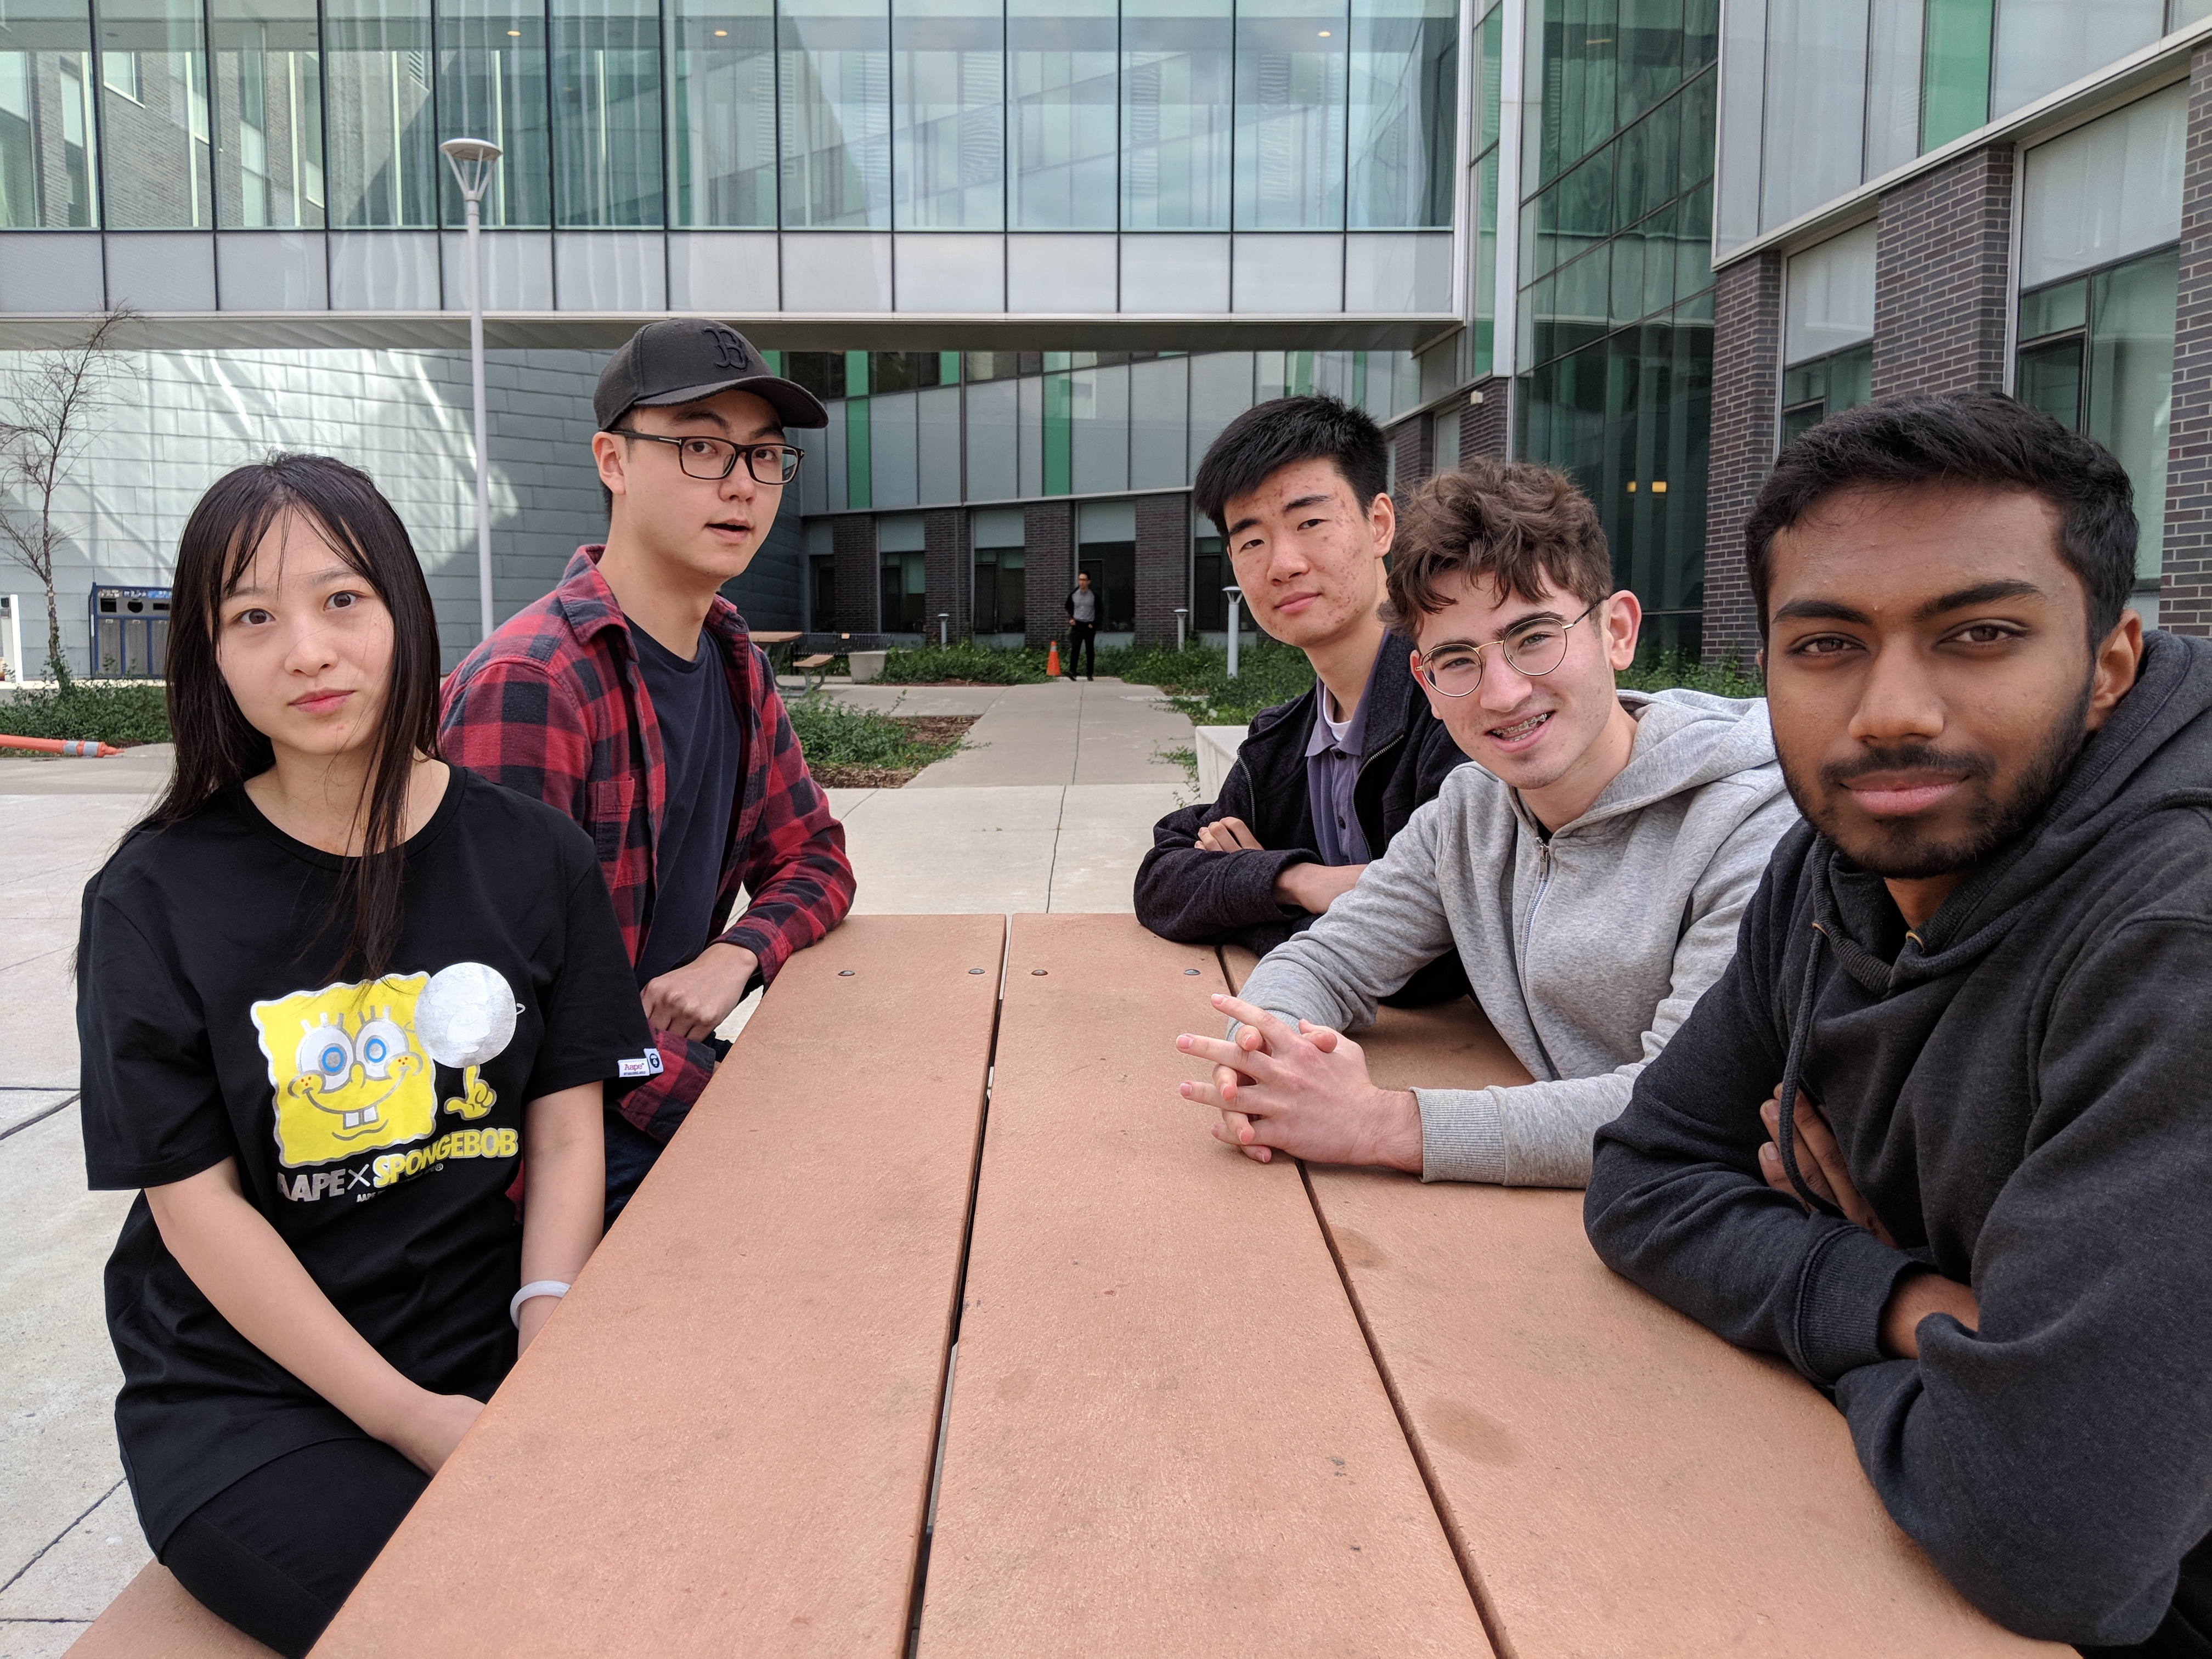
\includegraphics[width=0.9\textwidth]{team.jpg}
	\captionof{figure}{Photo of the whole team}
	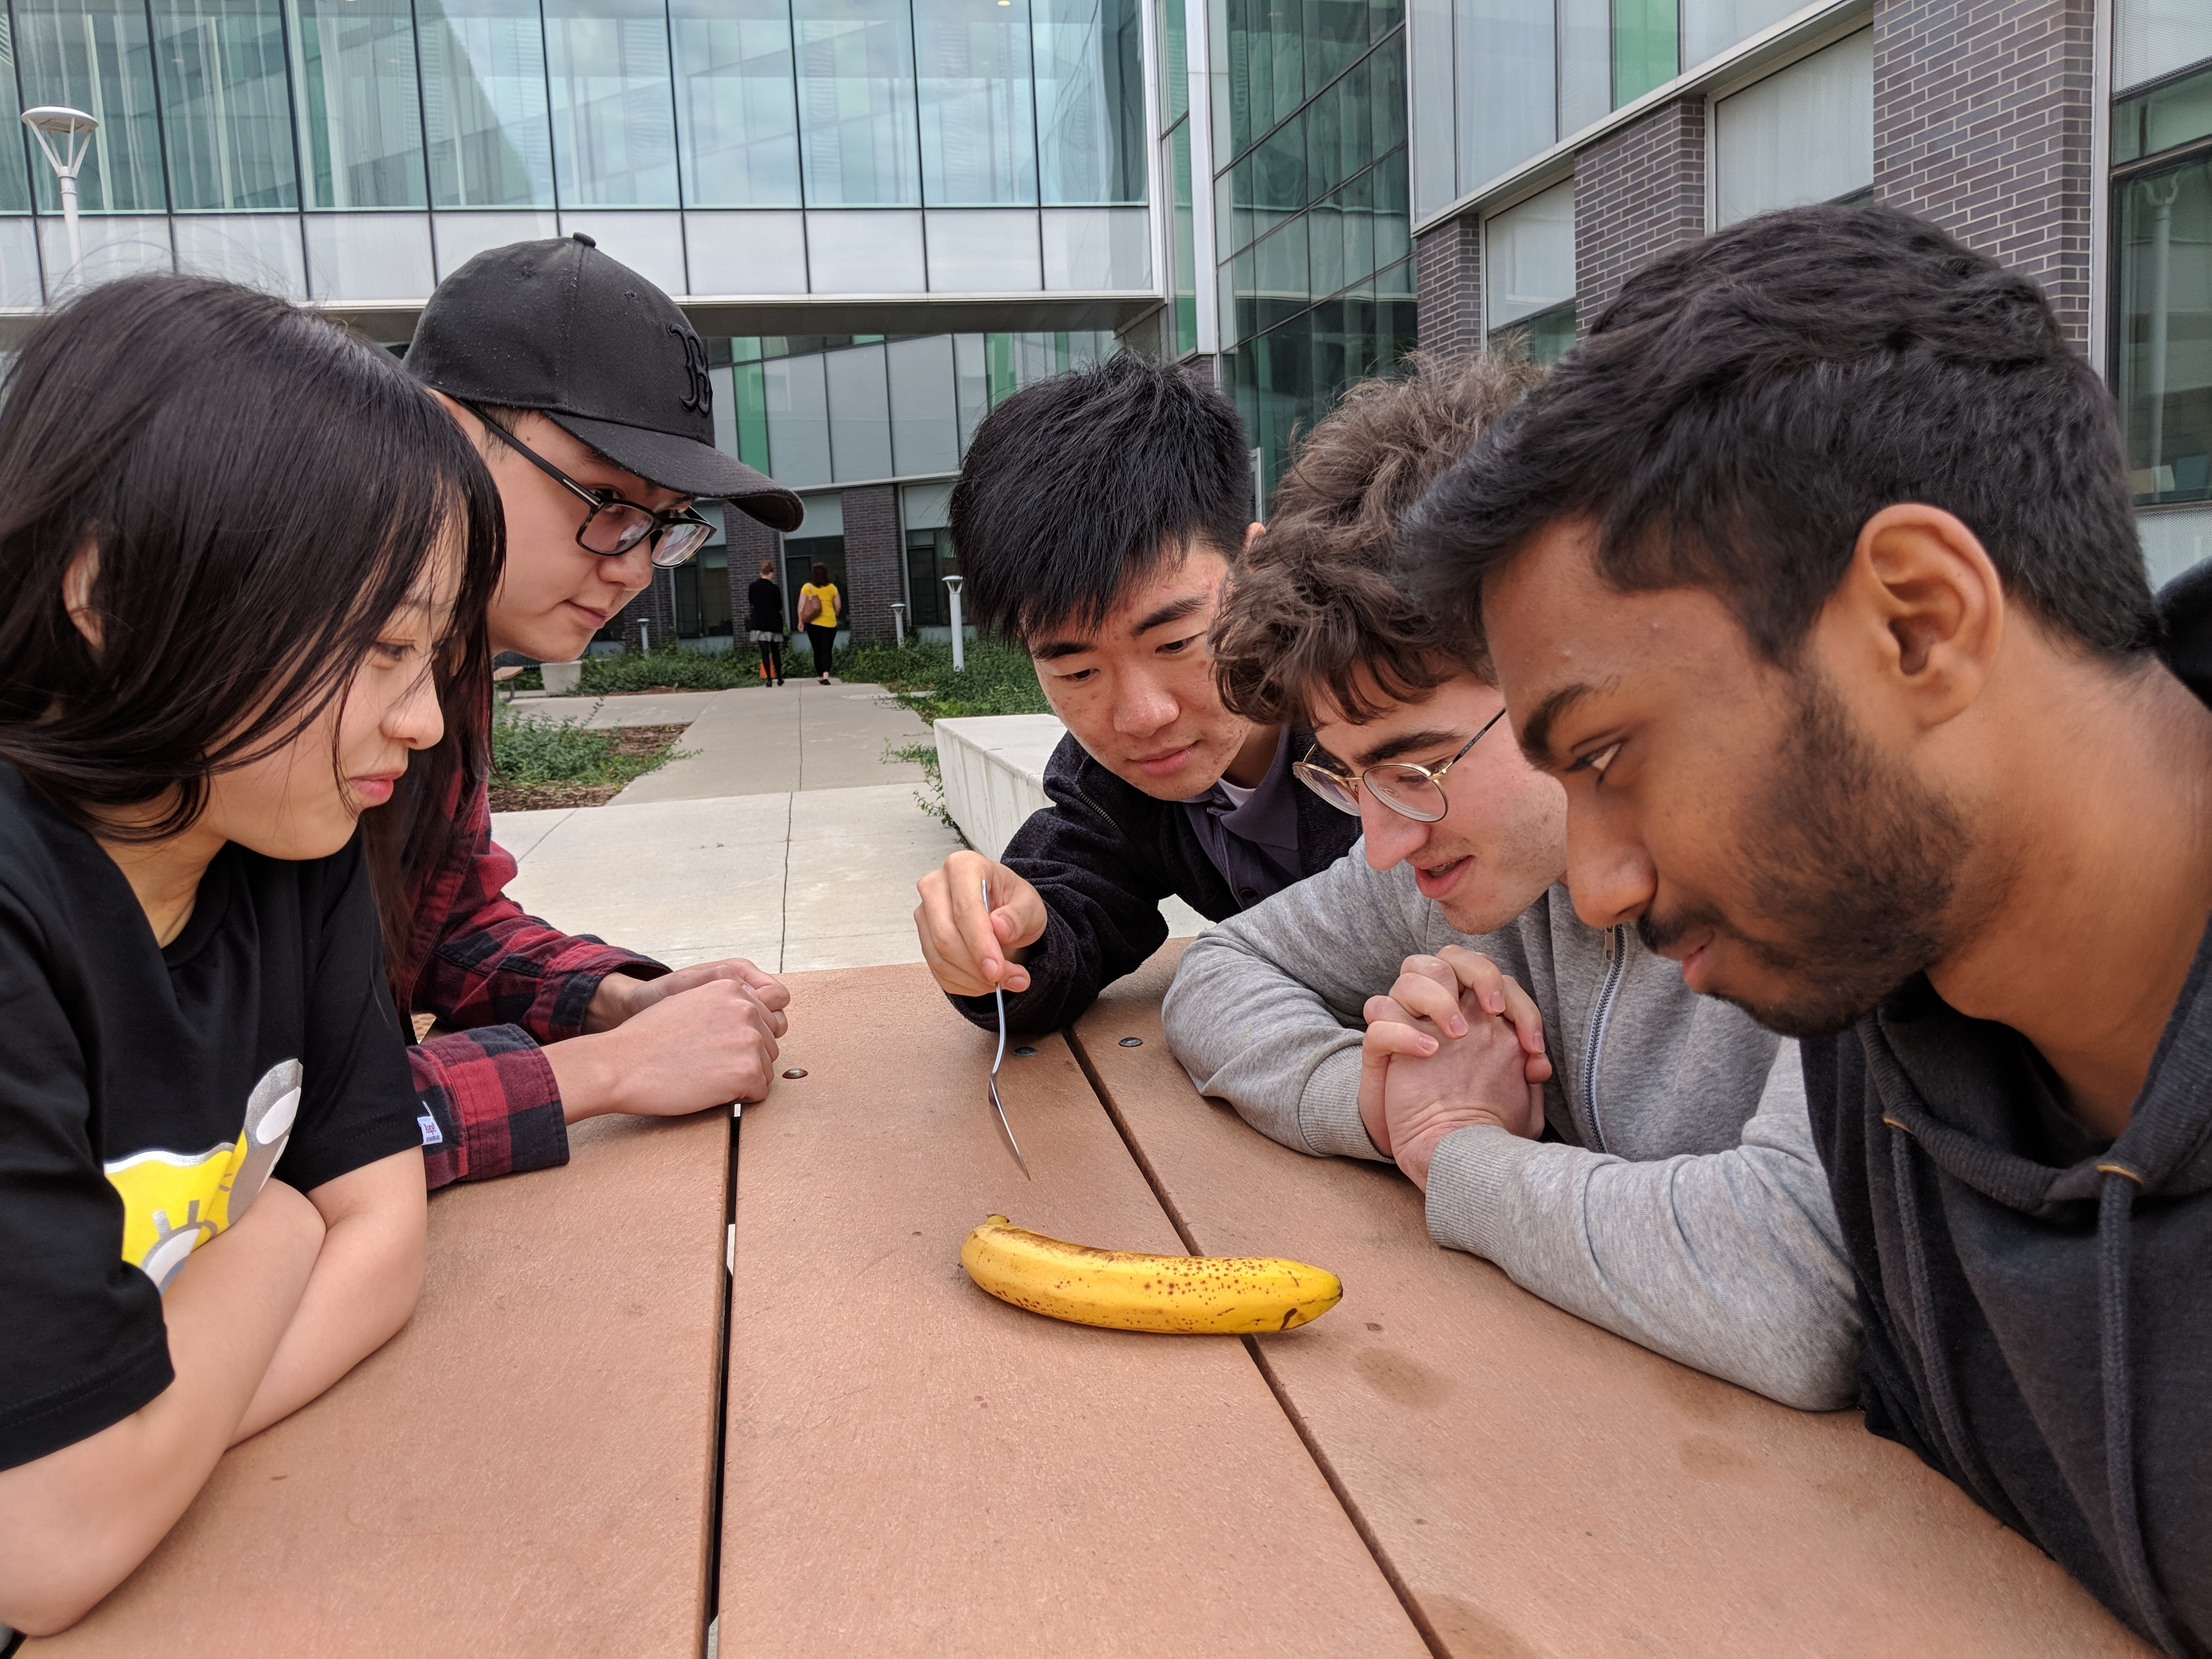
\includegraphics[width=0.8\textwidth]{food1.jpg}
	\captionof{figure}{Photo of team anticipating the consumption of a banana.}
	\vspace{0.5cm}
	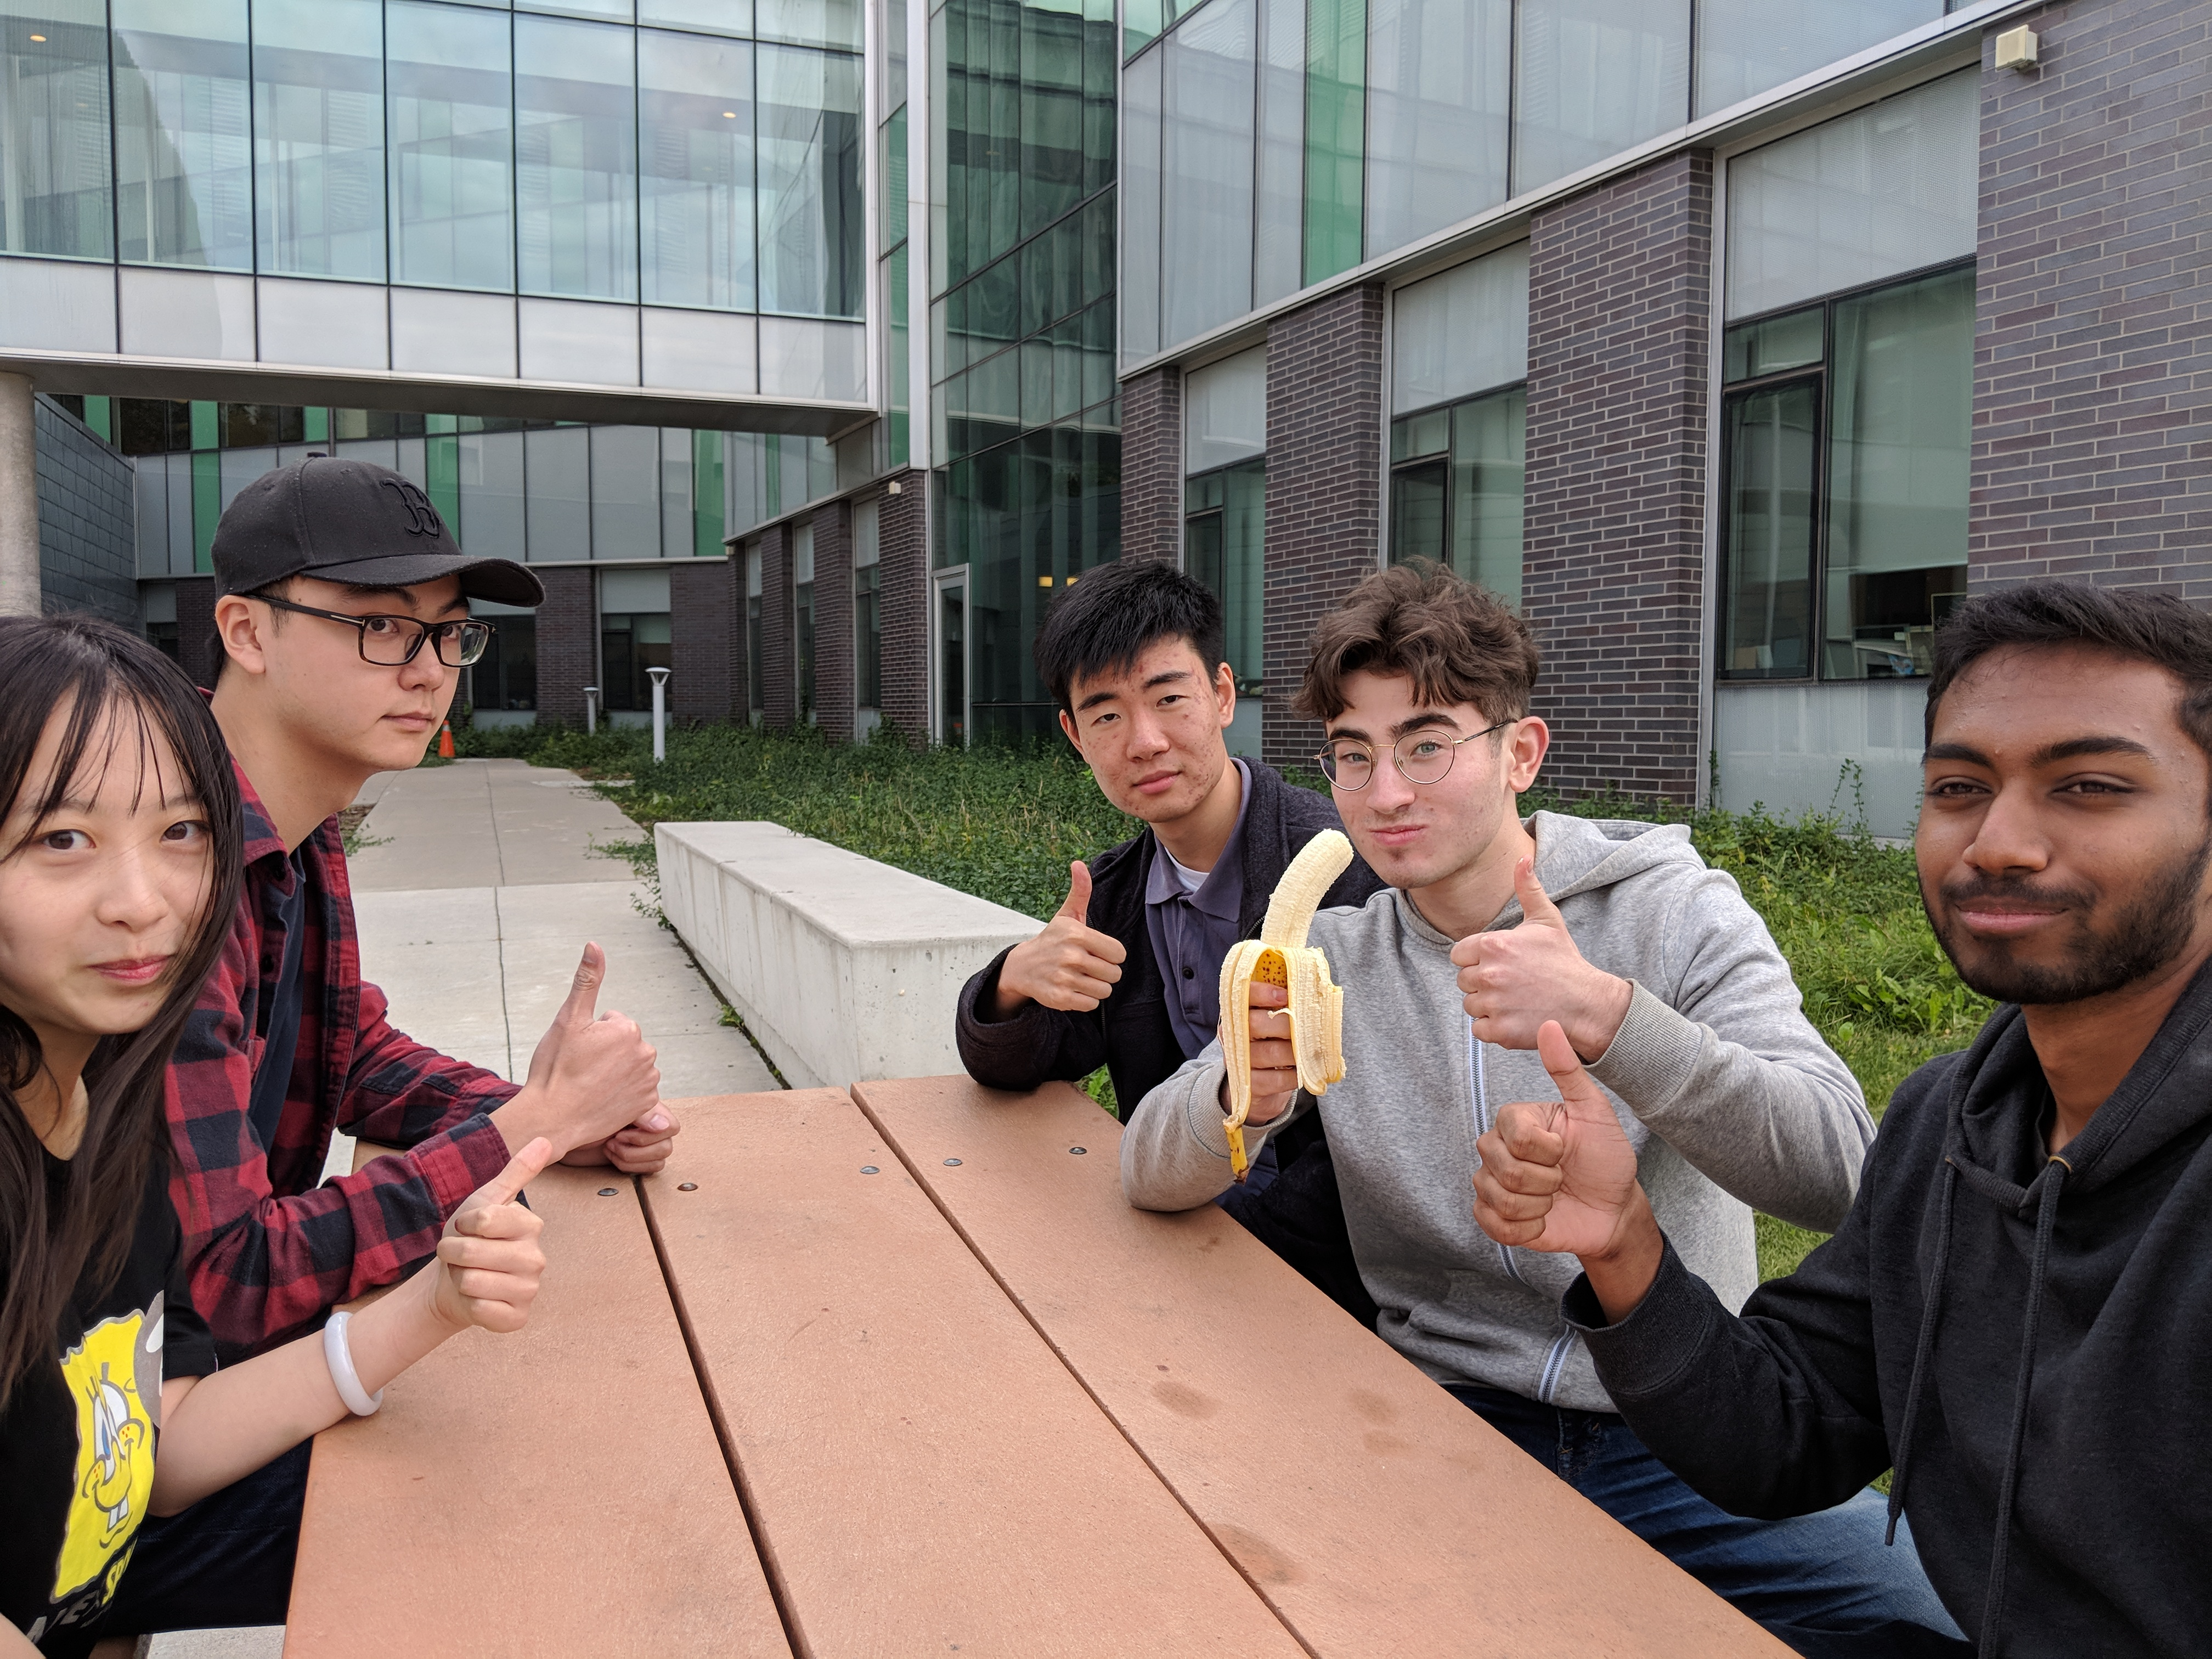
\includegraphics[width=0.8\textwidth]{food2.jpg}
	\captionof{figure}{Consumption of banana.}
\end{center}

\subsection{Our goals}
Our team has decided on a very specific set of goals. We list them below.
\begin{enumerate}
	\item Create a product that exceeds client expectations
	\item Use Agile practices to be an efficient, productive and organised team
	\item Improve existing skills and knowledge of software tools
	\item Learn new technologies and gain experience using them
	\item Establish rapport with client to have productive discussions of requirements
	\item Develop understanding of client needs to predict and anticipate features
\end{enumerate}

\subsection{Our strengths}
We are a diverse group of individuals, each with unique skills and experiences that help push at the boundaries of what we can achieve. Collectively, our team speaks 7 different languages: English, French, Spanish, Russian, Mandarin, Cantonese and Japanese. With each language comes a deep knowledge and understanding of the people who speak it, and their culture. This will help us create products that have much more target users, and as a result more active users.

We are good with people, but even better with technology. The whole team is fluent in Java and Python, and have experience using them in large software projects. A few of our team members know how to set-up and use databases, enabling us to add more complex features to our software. Not only have we used these skills for course work, but also in real work environments. Two of our team members, Jeffrey and Ashley have completed coop work terms. Jeffrey was a QA intern at OPS (Ontario Public Service), and Ashley completed a QA intern-ship at OTTP (Ontario Teachers' Pension Plan). Together, they bring in a year's worth of expertise in the public service field. Their experience and wisdom will be invaluable for our teams' success. 

We are skilled individually, but even more as a team. All of us have had experience working in Agile teams during B07. Some of us have also had Agile experience during coop work-terms. Agile knowledge will help us squeeze out as much as possible from our team.

Finally, the team has no known food allergies. We have yet to figure out how this is relevant to our project, but we are certain that it will prove useful in the future.
\newpage

\section{Meet the team}
\begin{wrapfigure}{l}{0.4\textwidth} 
	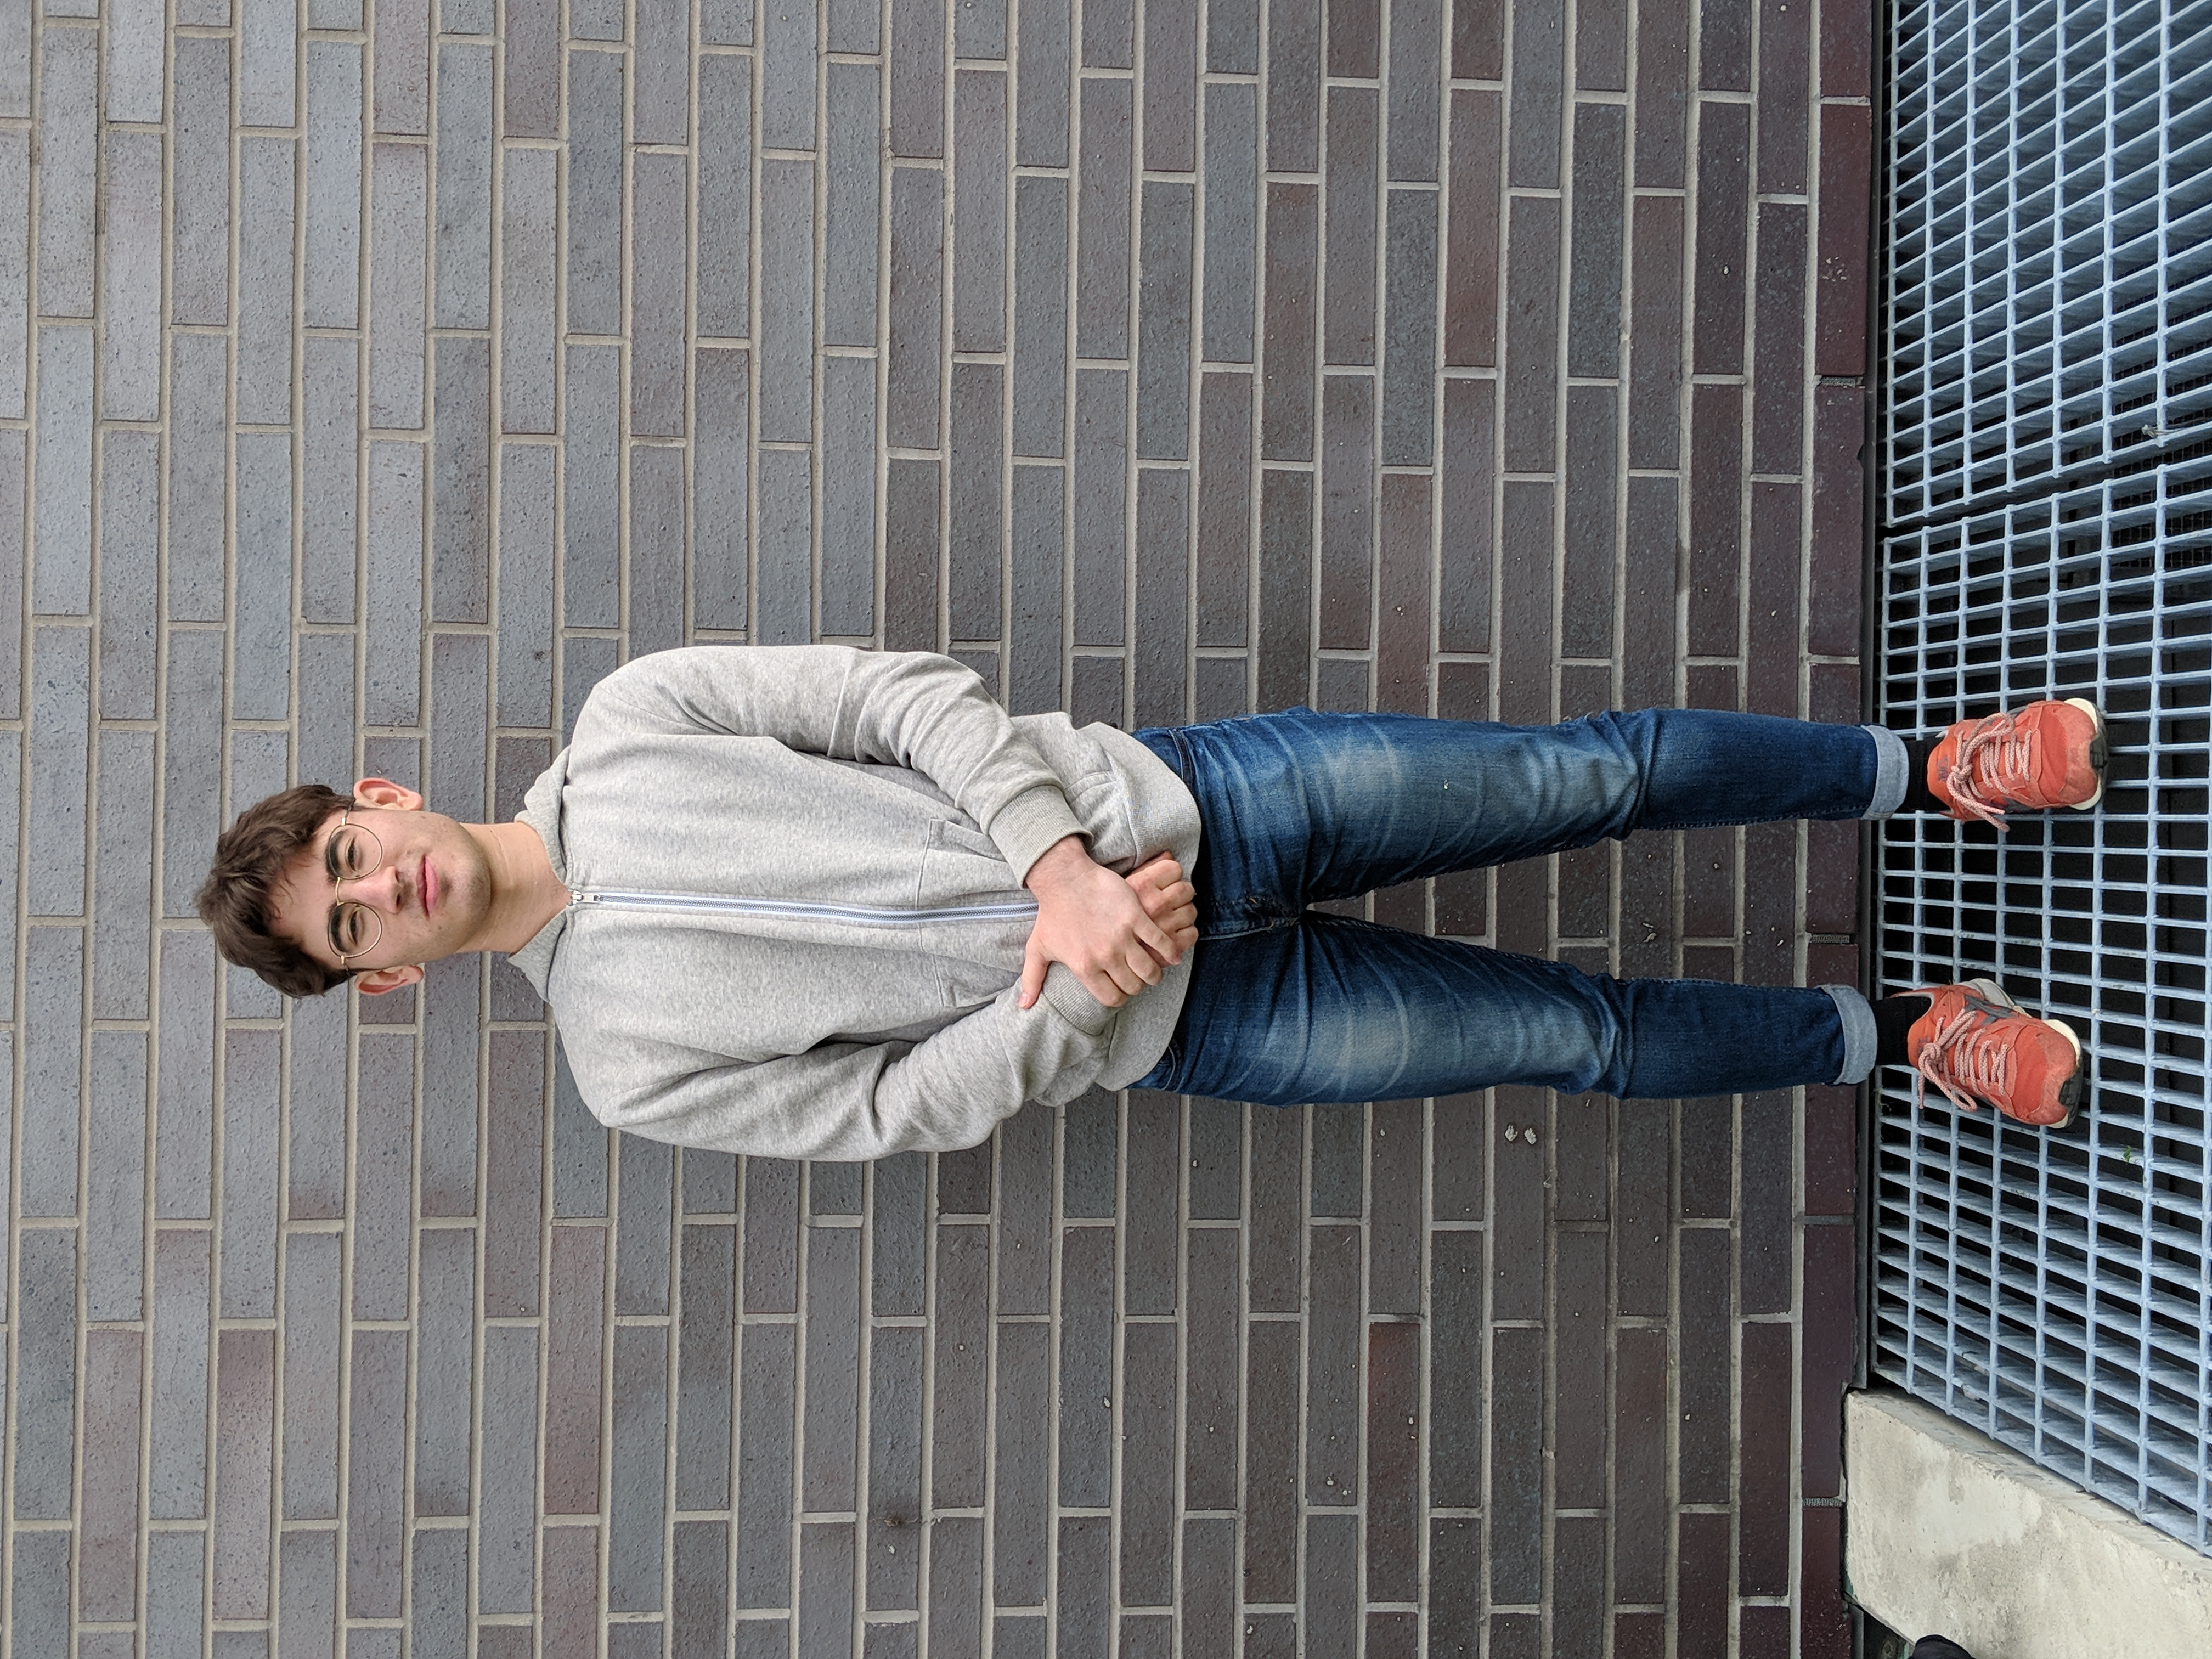
\includegraphics[angle=-90,origin=c,width=0.4\textwidth]{anton}
	\captionof{figure}{Anton}
\end{wrapfigure} 
I'm \textbf{Anton}, a second year CS student at UTSC. I have been interested in CS for as long as I can remember. I think of computer science and computer programming as an art, I like seeing and creating beautiful solutions to complex problems. I think CS is a good career path because it is useful in many industries. It excites me that I can see something I built or helped build being used by millions of people around the world to make their lives more enjoyable. Liking CS is one thing, but building good software is another. I have built a lot of software in my life, but the thing that stands out the most to me is an Android app for checking marks that I developed for high school students. It was a good challenge for me because I had to find sensible solutions to complex problems like data retrieval, sanitation and had to design a clear and intuitive UI for displaying the data. Although I like CS, it isn't the only thing I spend time on. I also enjoy playing soccer, flying drones, and typesetting anything I can in \LaTeX.\\


\begin{wrapfigure}{r}{0.4\textwidth} 
	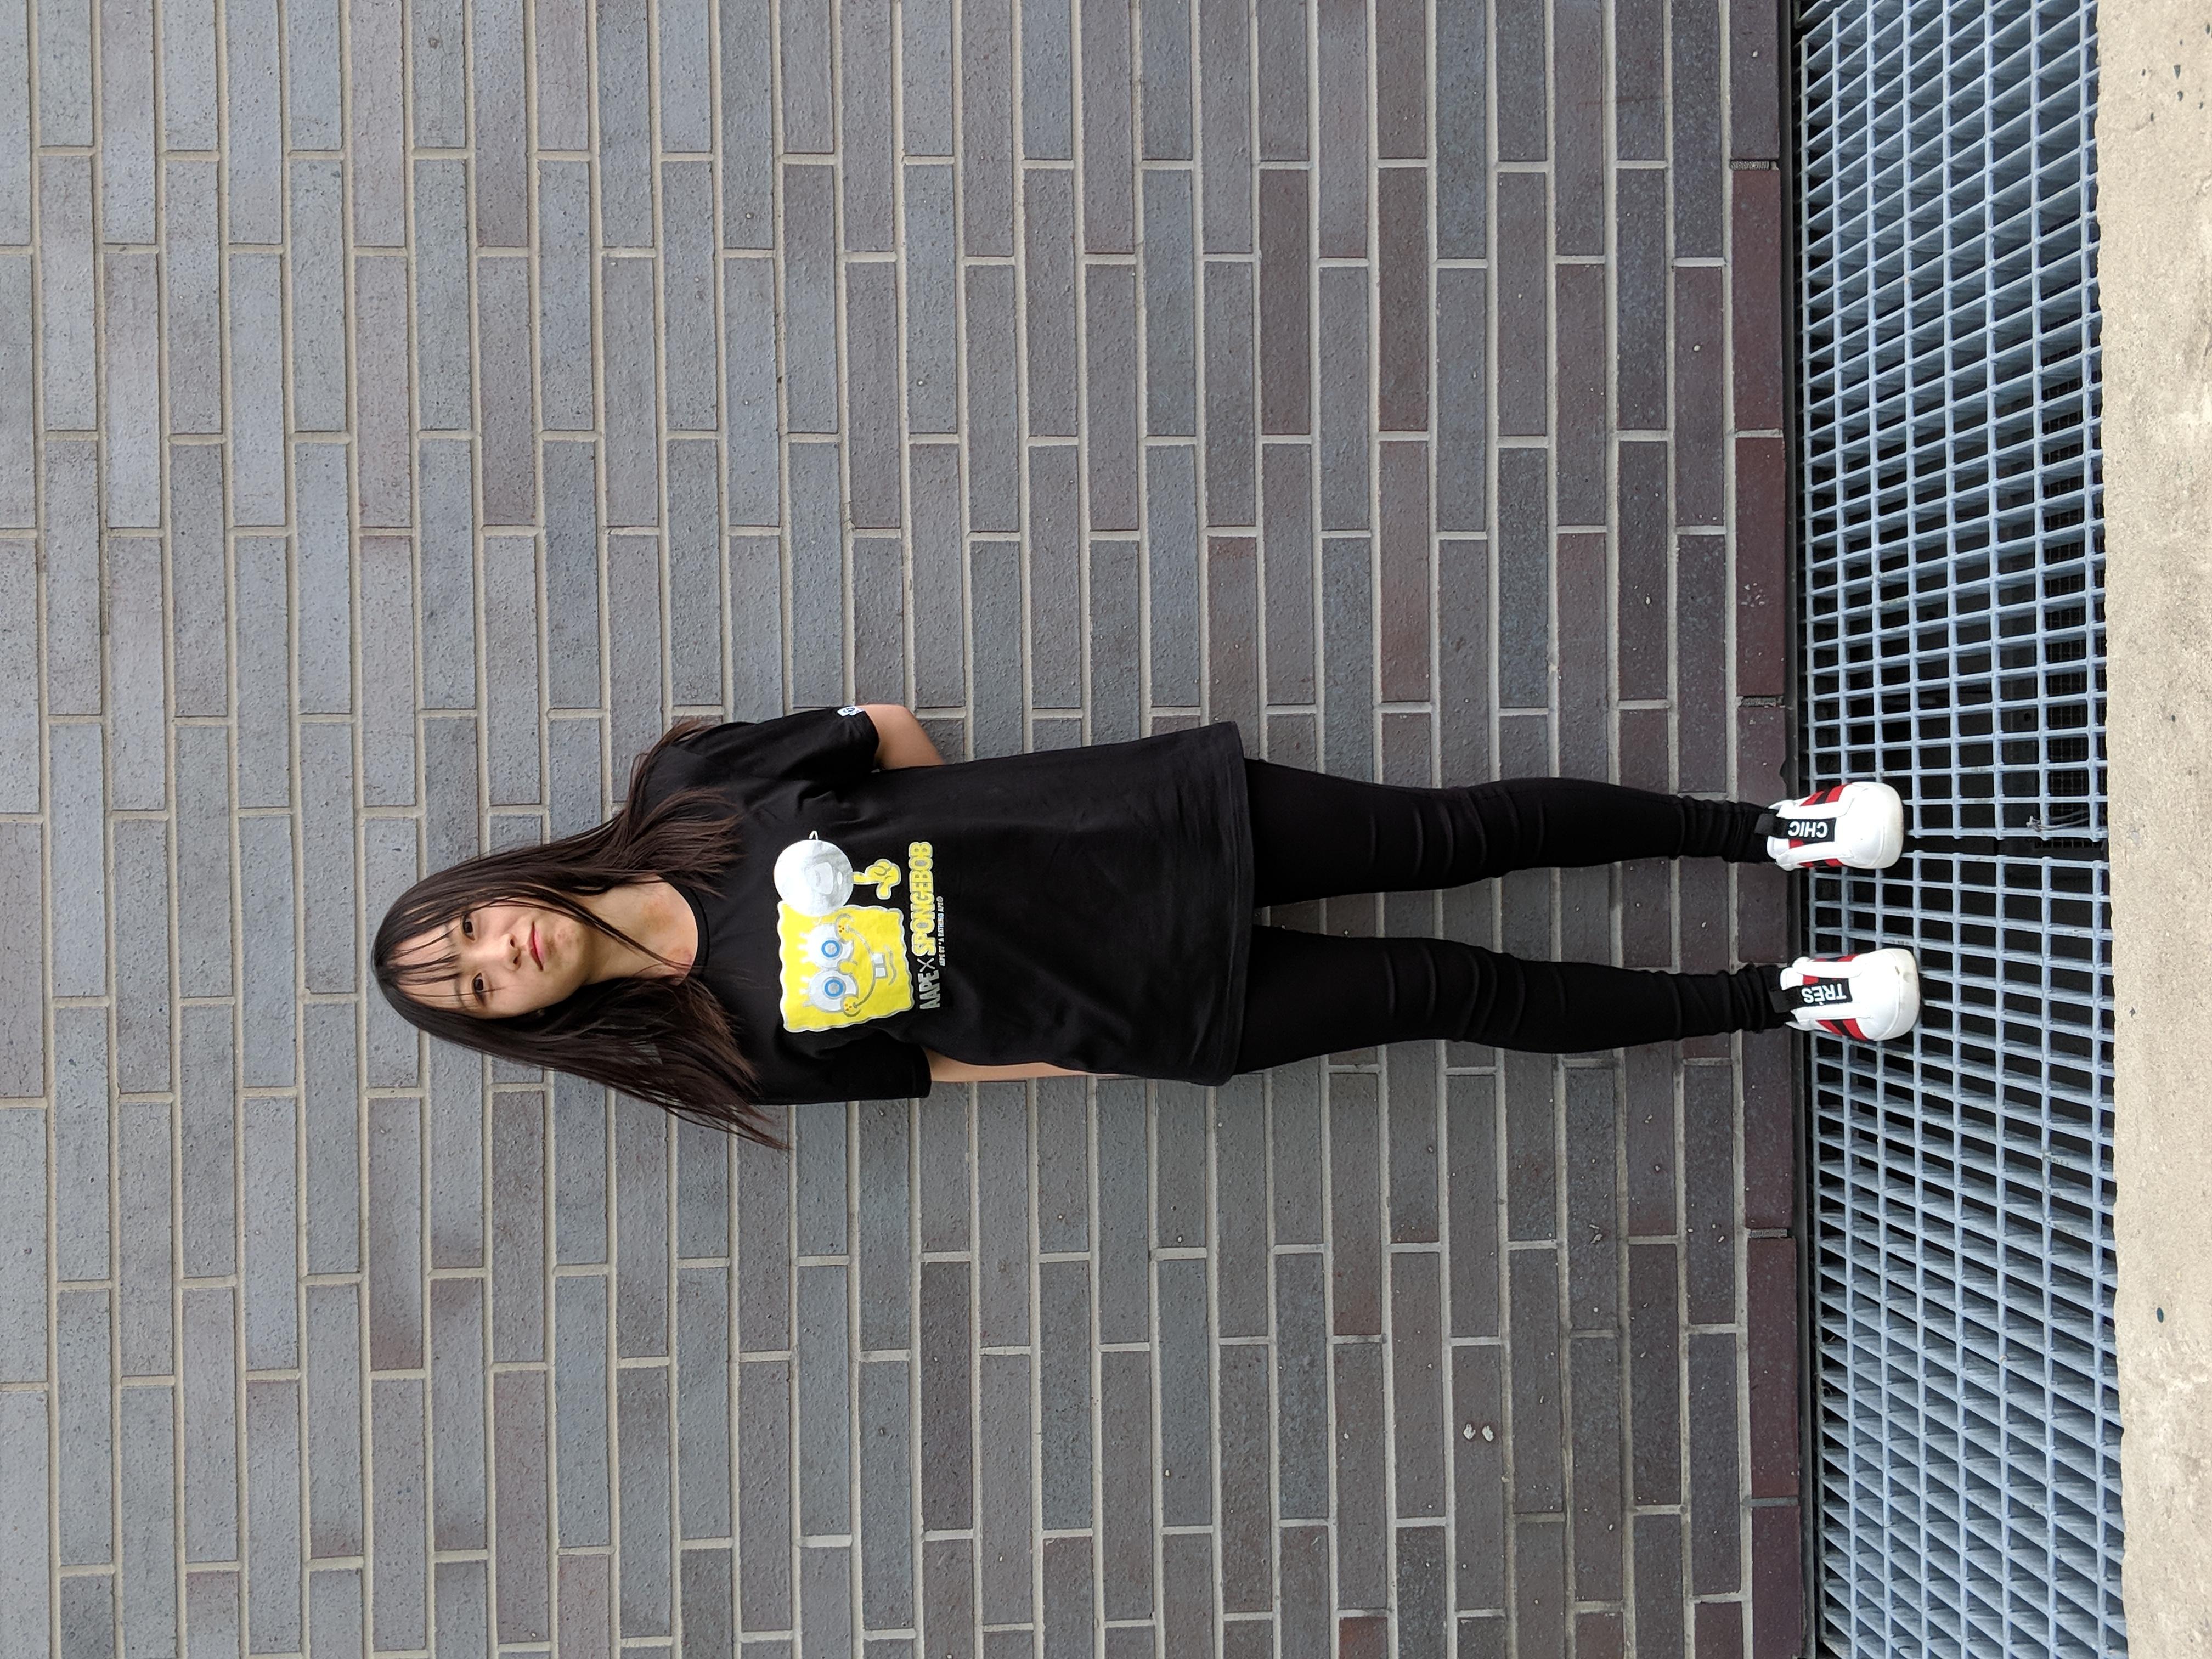
\includegraphics[angle=-90,origin=c,width=0.4\textwidth]{ashley}
	\captionof{figure}{Zifan}
\end{wrapfigure} 
\noindent Hi! I'm \textbf{Zifan}, a fourth year student studying in the CS management specialist program. I chose this stream because I have interest in Computer Science but also want to learn management. My technical skills are basic Python, Java, C, CSS and PHP. My favourite CS project was a group project for CSCB07. We used Java to build an Android app for online shopping. It had login functionality and added shopping records to a database. I enjoyed working on this project because I had a really good team, who all did an equal share of work. During my leisure time I like to practice Chinese calligraphy, swim and watch Japanese Anime. I am Chinese but I have studied Japanese for 6 years, so I am fluent in Japanese. I got an offer from Waseda University (a University in Tokyo, Japan) back in 2012, but I chose not to go because of the big earthquake that year.\\\\

\begin{wrapfigure}{l}{0.4\textwidth} 
	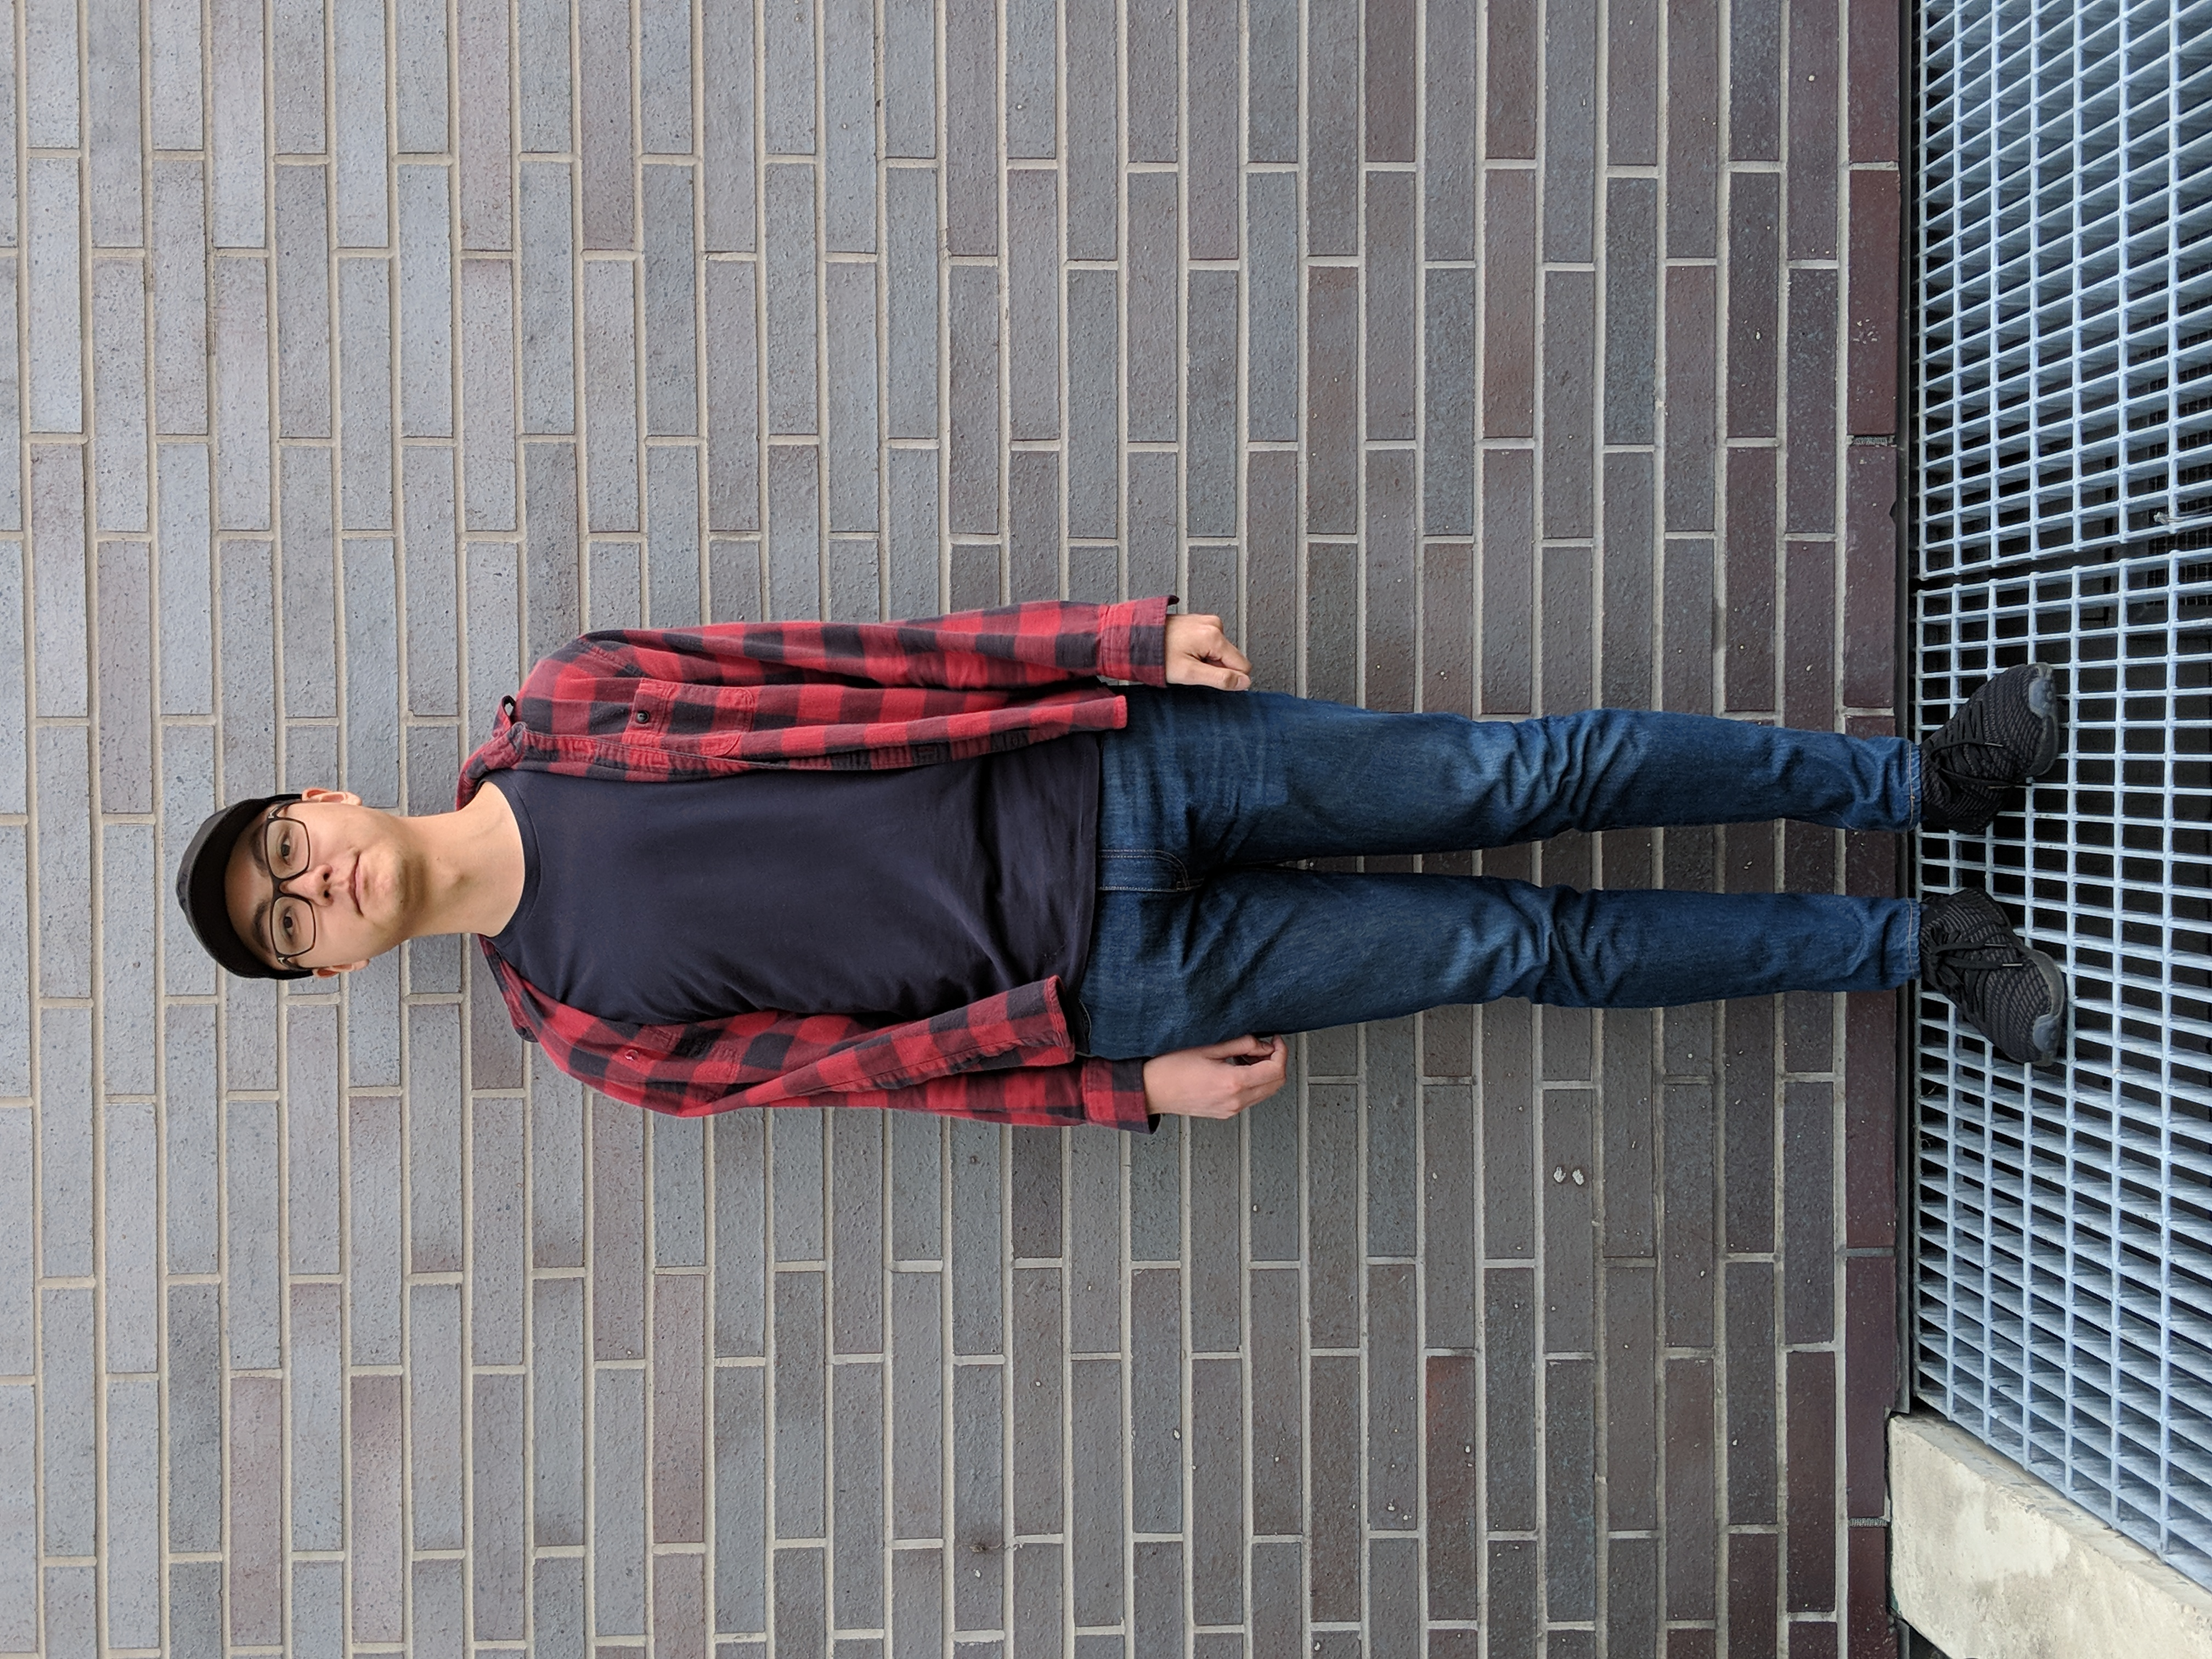
\includegraphics[angle=-90,origin=c,width=0.4\textwidth]{kelvin}
	\captionof{figure}{Kelvin}
\end{wrapfigure}
\noindent Hi, my name is \textbf{Kelvin} and I am a third year Computer Science student in the software engineering stream. I have experience with Java, C, Python and Android app development. I chose Computer Science because of my interest in computers and programming. My favourite CS project was for CSCB58 because we were given few project requirements. My team created a Casino app on a DE2 board that could play Blackjack, roulette and slots. We used the on board LEDs as output and the switches for user input. You were able to switch between games, and the board kept track of the scores. My hobbies are headphones, watching anime and building Gundam model kits.\\\\\\\\

\begin{wrapfigure}{r}{0.4\textwidth} 
	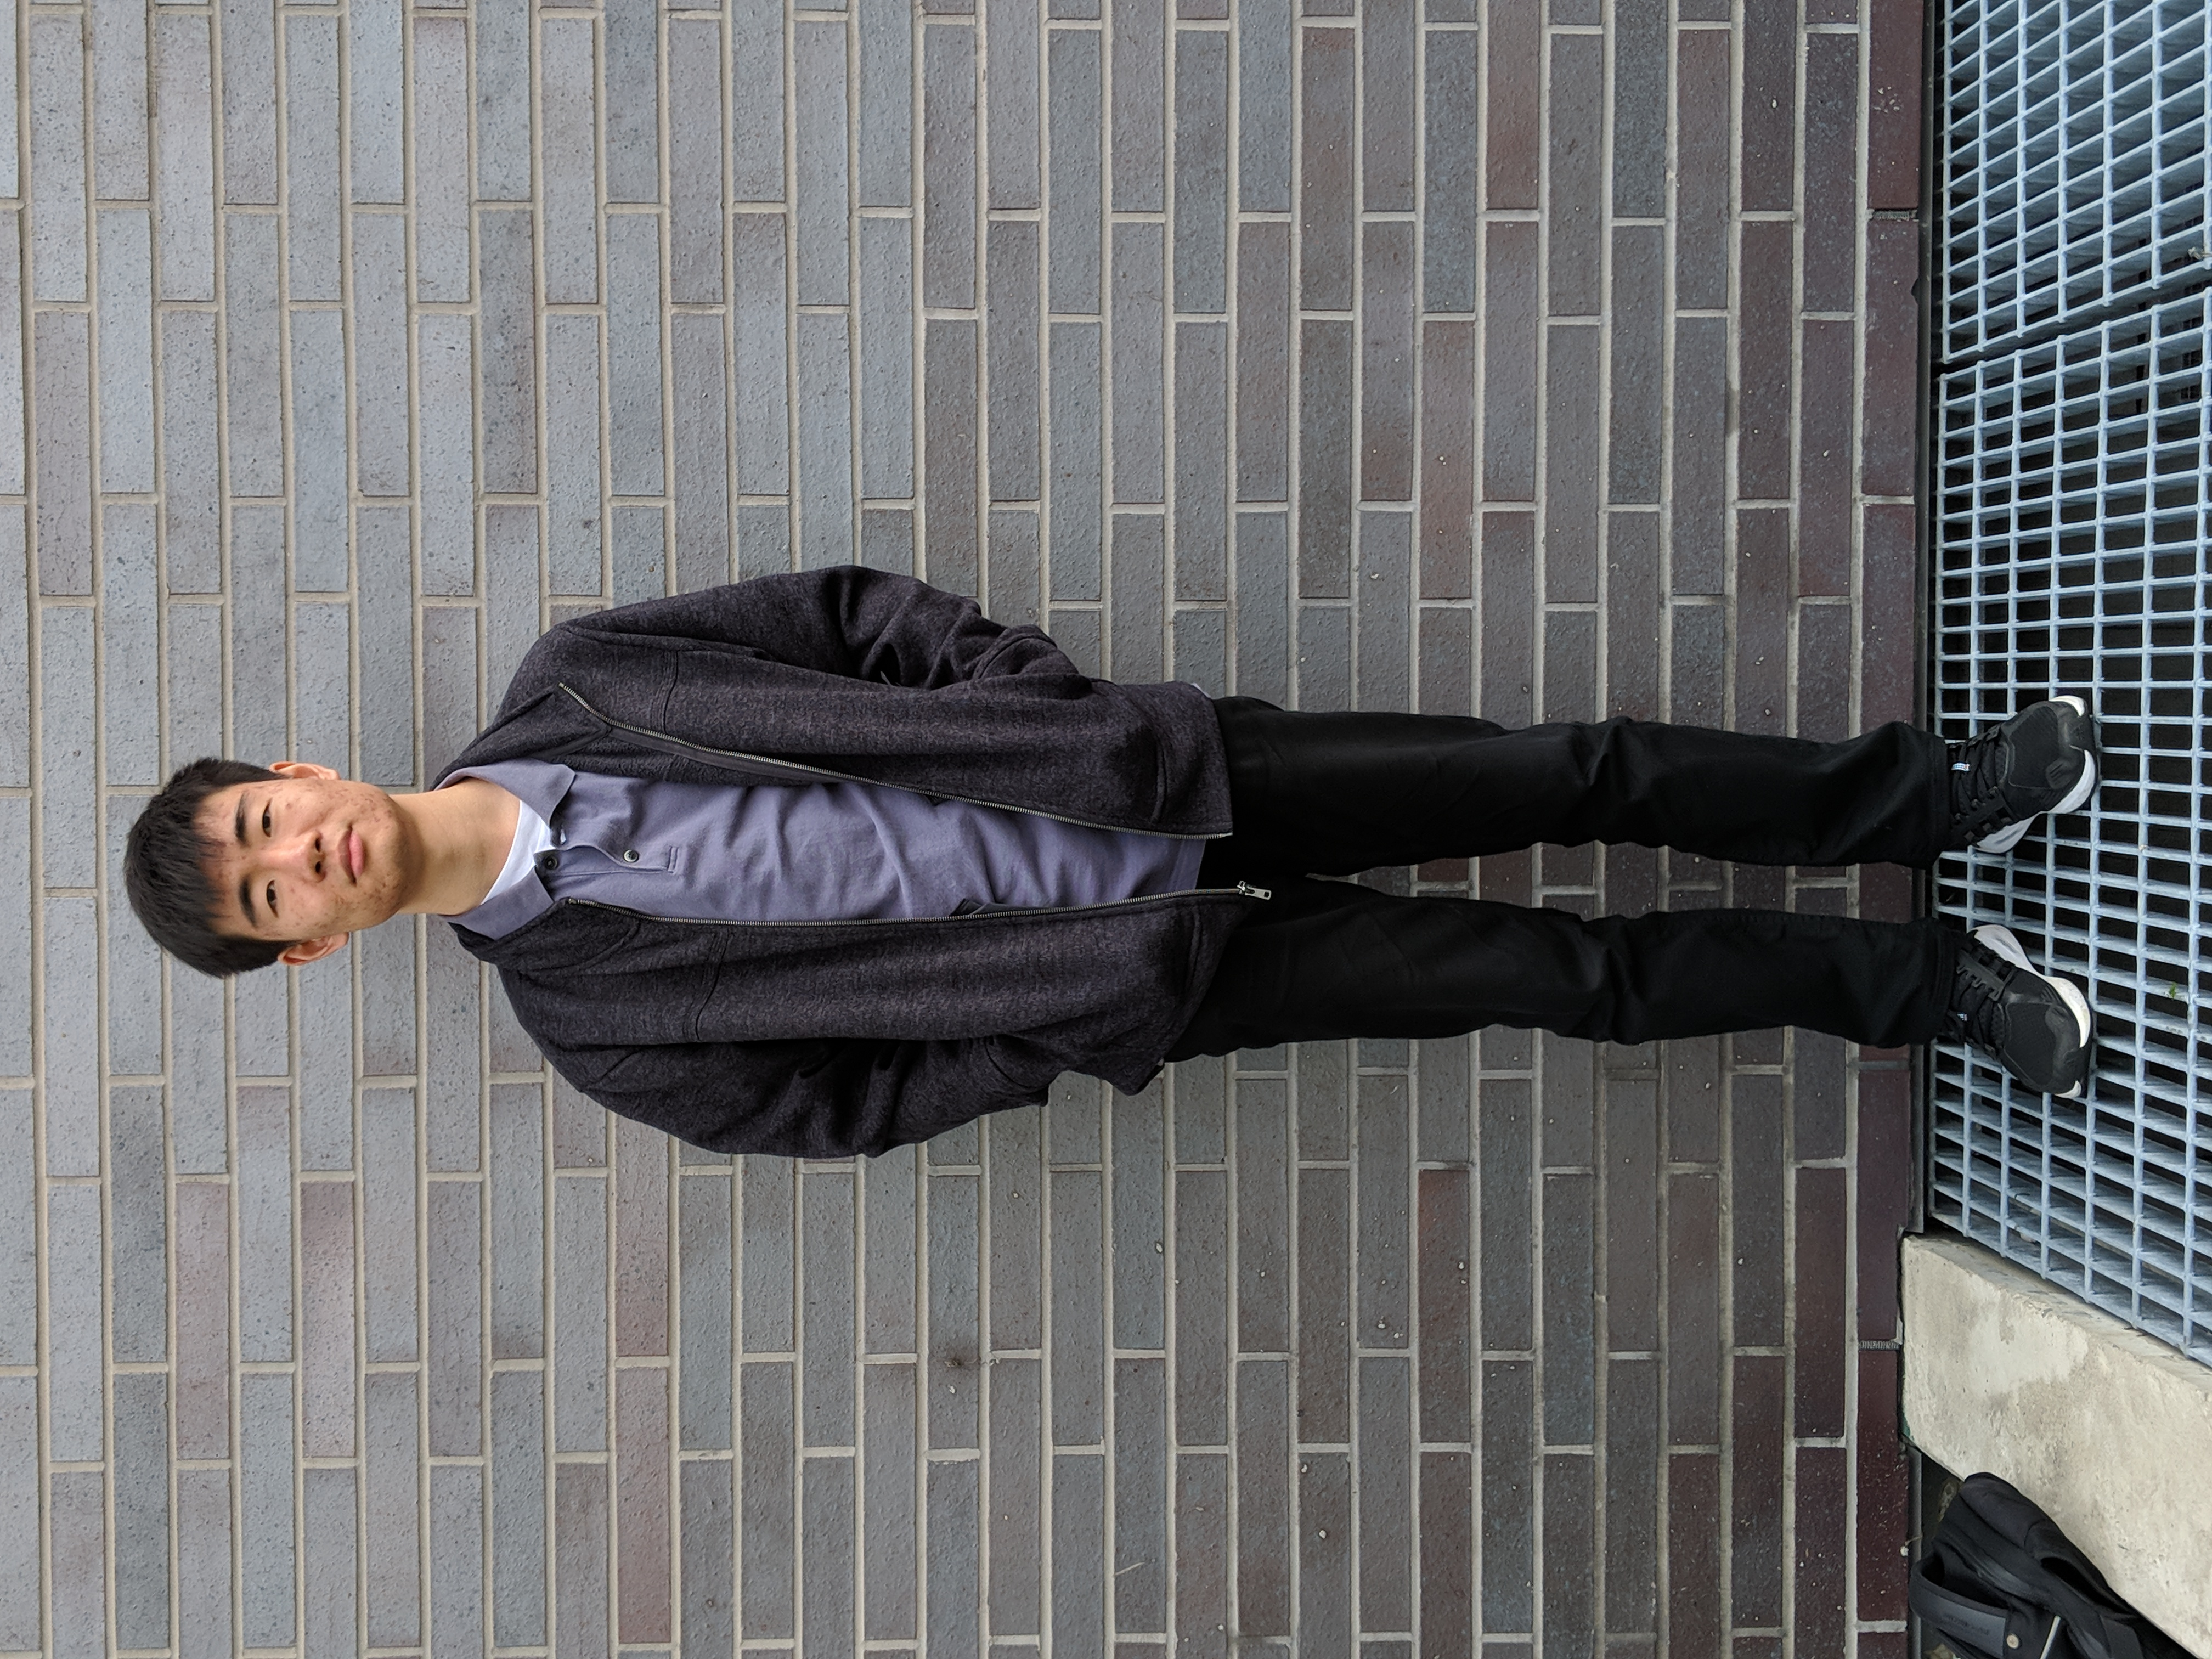
\includegraphics[angle=-90,origin=c,height=3in]{jeff}
	\captionof{figure}{Jeffrey}
\end{wrapfigure}
\noindent Hello there! My name is \textbf{Jeffrey}, I am a third year undergraduate in software engineering. I have always had an interest in computer science since high school, having developed Windows applications and games in Visual Basic, and participated in coding competitions and hackathons.  I am proficient in Python, Java, and C\#. From my previous QA experience with the Ontario Public Service, I have some basic understanding of database design and the different types of software testing. As an OPS QA, I led the development of an automation framework based in Selenium coded in C\#, where I took part in scrum meetings and pair coding sessions. I really enjoyed the idea of developing a system to be used by future QAs. My current hobbies are photoshopping and making videos with Sony Vegas. In fact, I was the main video editor for my FRC robotics team back in high school. I also like to play strategy and FPS video games, surf YouTube and Reddit, and edit wiki articles from time to time.

\begin{wrapfigure}{l}{0.4\textwidth} 
	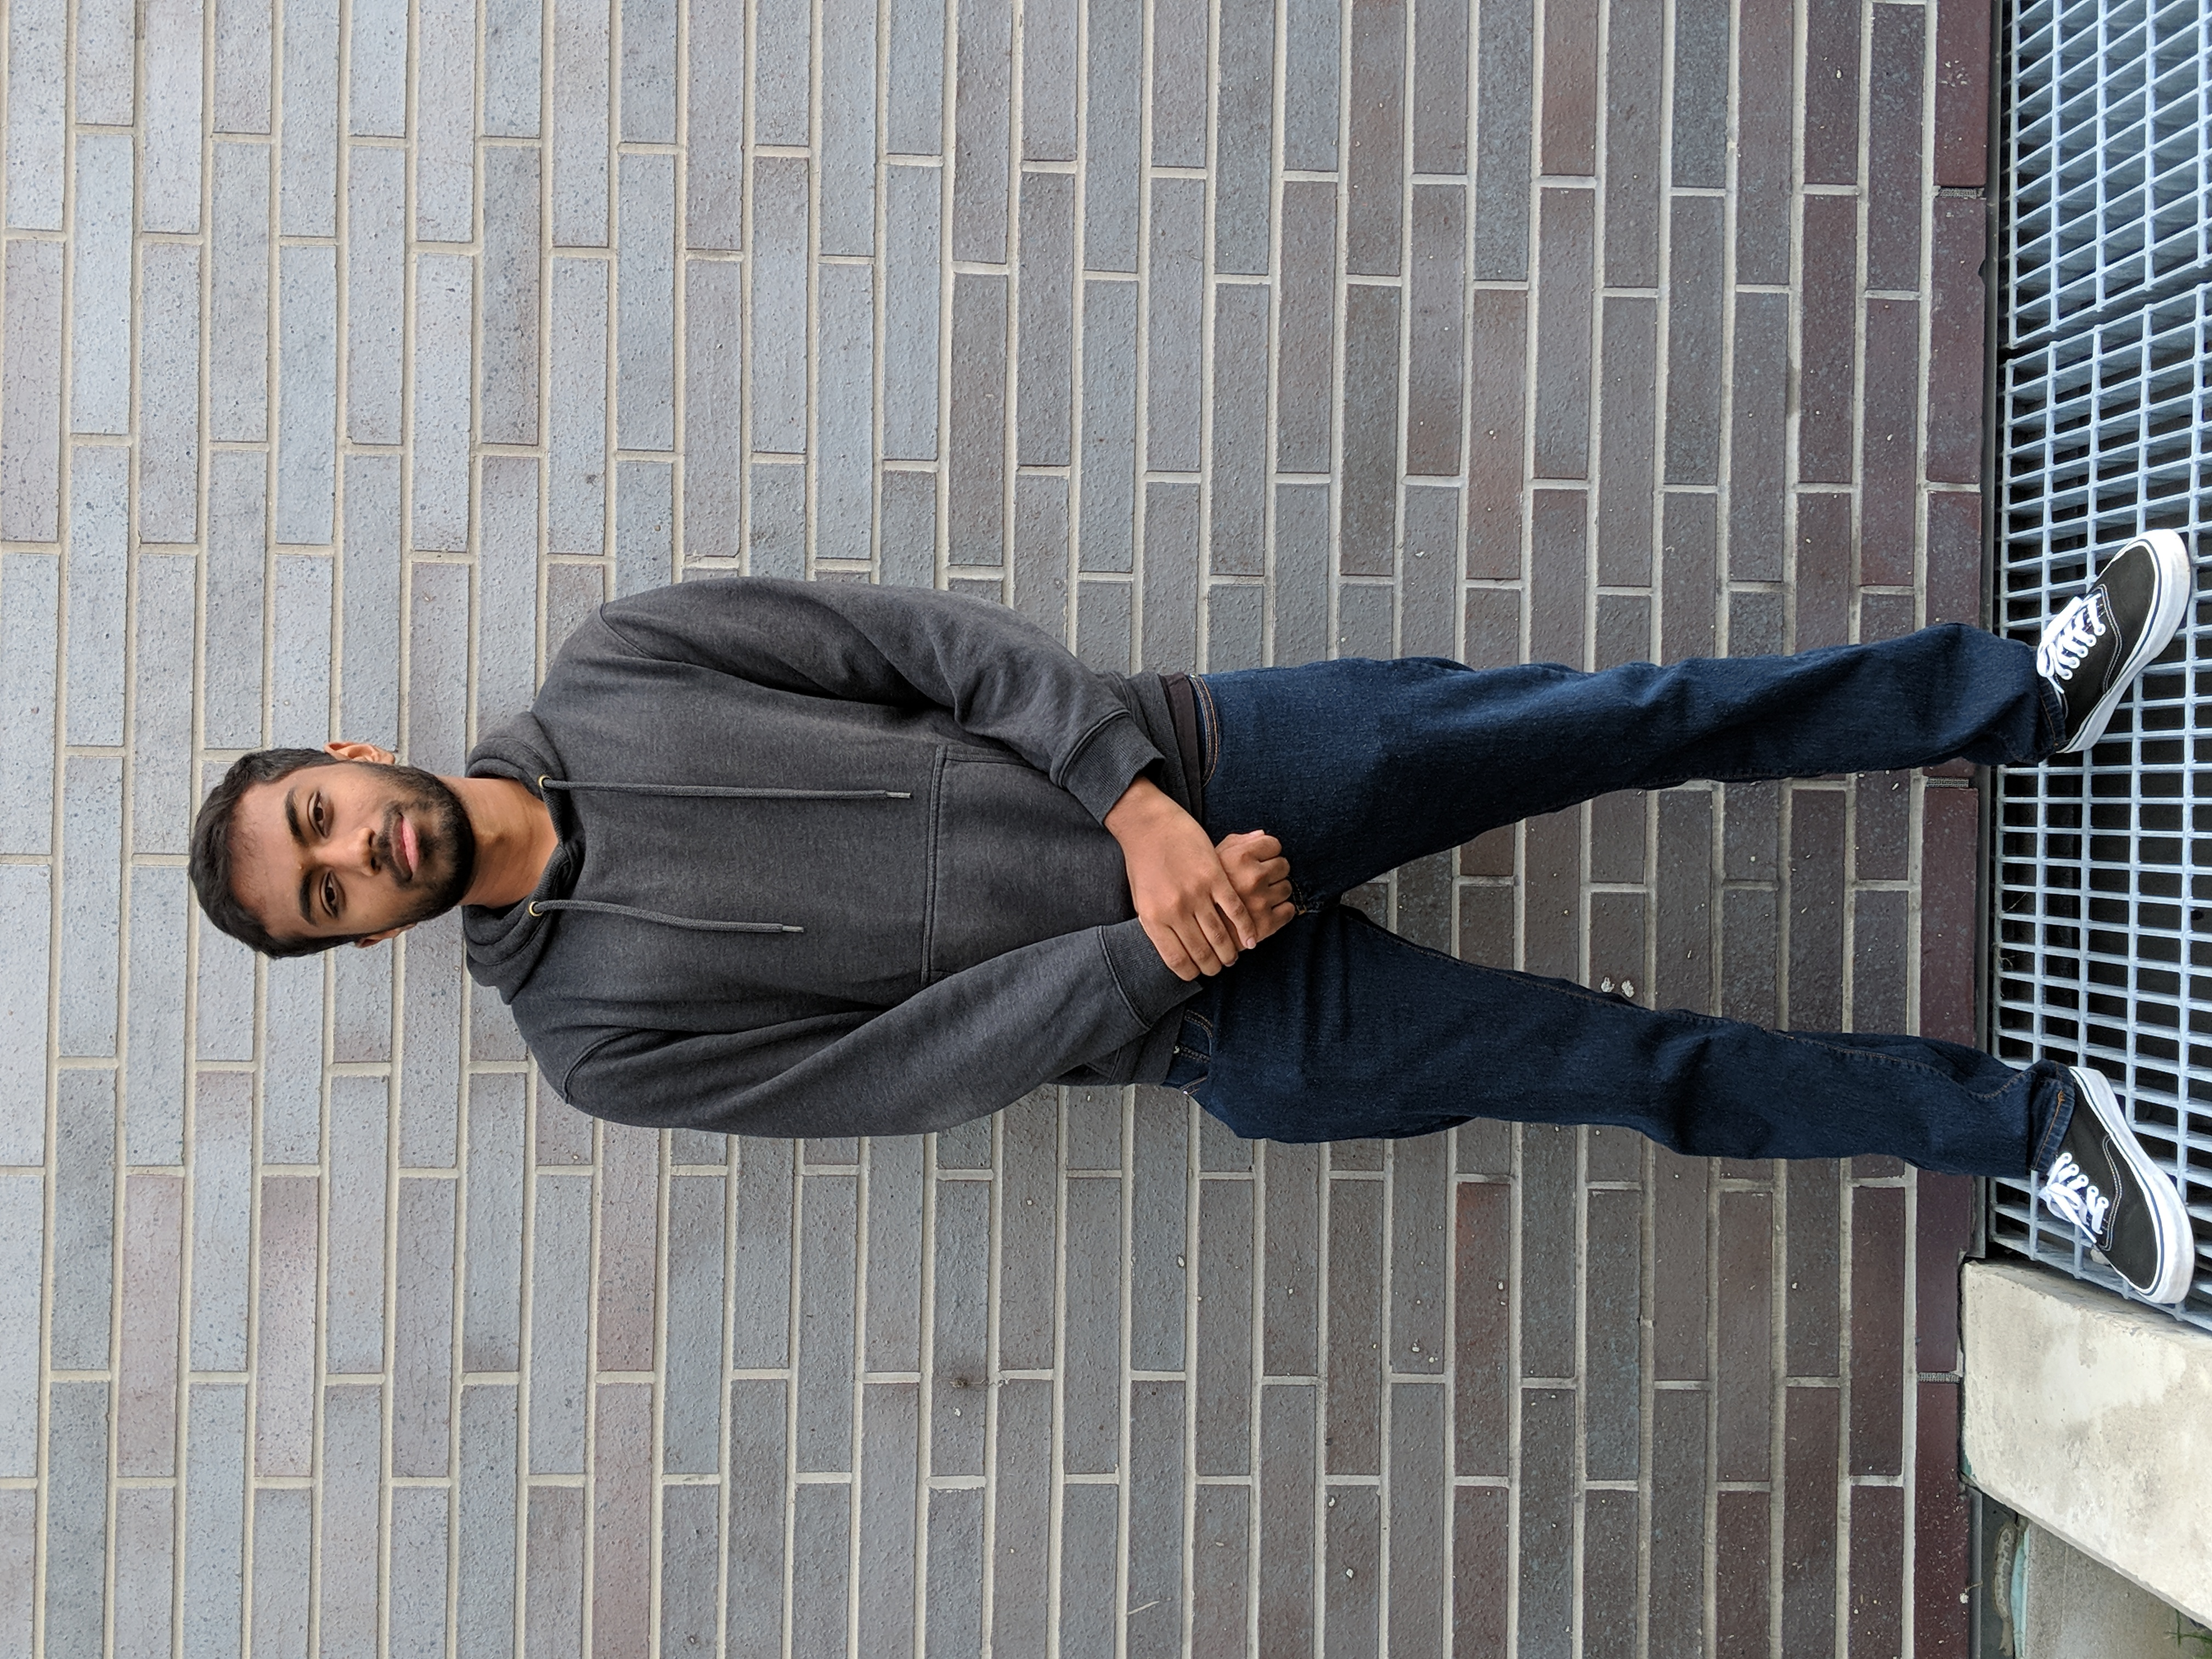
\includegraphics[angle=-90,origin=c,width=0.4\textwidth]{christian}
	\captionof{figure}{Christian}
\end{wrapfigure}
My name is \textbf{Christian}, and I am a third year student studying CS Data Mining and Machine Learning specialist. I choose this program because I enjoy programing and I am fascinated by machine learning. The programing languages I’m familiar with include Python, Java, C and I have working knowledge of HTML and SQL. My favorite project to have worked on was the final project for CSCB58, where in groups of two, we were to develop any product of our choice, using Verilog. We developed a multi leveled two player game, with scaling difficulty. I enjoyed the creative freedom of this project, and working in a new language no one was familiar with. During my spare time I like to weight train, watch UFC, play competitive video games and watch anime.




\end{document}          
